\documentclass[a4,12pt]{scrartcl}

%Basic 
\usepackage[utf8]{inputenc}
\usepackage[ngerman]{babel}
\usepackage[T1]{fontenc}
%Schrift 
\usepackage{textcomp} % Für μ \textmu
%\usepackage{fontspec} 
%\setmainfont{Arial} 
%Zeilenabstand
\usepackage{setspace}
\setstretch {1.3}
\usepackage{float}
\usepackage[bottom = 3.50cm]{geometry}

%Titel Seite
\usepackage{titling} %Wird benötigt damit \maketitle die Variabeln title, author und date nicht überschreibt
\title{Usability-Test}
\subtitle{Projekt: sniffdatel}
\author{David Meister \and Giorgio Vincenti \and Samuel Krieg \and Andreas Stalder}		
 %mit /and können Personen hinzugefügt werden
\date{\today}


%Kopf, Fusszeile
\usepackage{fancyhdr}
\pagestyle{fancy}
\lhead{SW Engineering Projekt FS 2016}
\chead{}
\rhead{sniffdatel}
\lfoot{\thetitle \: v1.0 }
\cfoot{\today }
\rfoot{Seite \thepage}
\renewcommand{\headrulewidth}{0.4pt}

%Bilder
\usepackage{graphicx}

%Zeichnen
\usepackage{tikz}

%Tabellen
\usepackage{booktabs}
\usepackage{longtable}

%Codesnippets
\usepackage{listings}
\lstset{language=java,basicstyle=\footnotesize,frame=single} %backgroundcolor=\color{lightgray}

%Querformat für eine Seite
\usepackage{lscape}
\usepackage{rotating}
\usepackage{pdflscape}

%URL 
\usepackage[colorlinks=true, linkcolor=blue, urlcolor=blue, citecolor=blue]{hyperref}
\urlstyle{same} 


%Loremimpsum
\usepackage{lipsum}



\begin{document}

%\clearpage\maketitle
\begin{titlepage}
	\centering
	\vspace{5cm}
	\begin{center}
	
\includegraphics[width=0.50\textwidth]{logo.png}
	\end{center}
	{\huge\bfseries sniffdatel\par}
	\vspace{8cm}
	\raggedright
	{\bfseries SW Engineering Projekt FS 2016\par}
	{\huge\bfseries Usability-Test\par}
	\vspace{1cm}
	{\theauthor \par}
	{\today\par}

\end{titlepage}

\section{Änderungsgeschichte}

\begin{table}[htb]
\centering
    \begin{tabular}{@{} l l l l@{}}\toprule    
    {Datum} & {Version} & {Änderung} & {Autor}\\ \midrule
    21.05.16 & 1.0 & Erstellung erster Version & Giorgio Vincenti\\ \addlinespace
    23.05.16 & 1.0 & Erste Testperson & Giorgio Vincenti\\ \addlinespace
    24.05.16 & 1.0 & Zweite Testperson & Giorgio Vincenti\\ \addlinespace
    24.05.16 &  1.0 & Dritte Testperson & Giorgio Vincenti\\ \addlinespace
    24.05.16 & 1.0 & Korrektur & David Meister\\ \addlinespace
    26.05.16 & 1.0 & Korrektur & Giorgio Vincenti\\ 
    \bottomrule
    \end{tabular}
\caption{\textbf{Änderungsgeschichte}}
\end{table}
\newpage
%\thispagestyle{empty}
\tableofcontents
\newpage

\section{Einführung}
\subsection{Zweck}
Dieses Dokument dient als Usability-Test Dokumentation für das Projekt \textbf{sniffdatel}. 
\subsection{Gültigkeitsbereich}
Das Dokument bezieht sich auf die Software \textbf{sniffdatel}, welche im Rahmen des Moduls Engineeringprojekt des Frühjahrssemester 2016 entwickelt wird und ist während des gesamten Projekts gültig. 
\subsection{Referenzen}
\begin{itemize}
\item doc/02\_projektplan/Projektplan\_v1.7
\item doc/03\_analyse/Anforderungsspezifikationen\_v1.1
\item doc/03\_analyse/Domainanalyse\_v1.1
\item doc/04\_design/Architektur\_v1.1
\item doc/04\_design/ExternesDesign\_v1.0
\item doc/05\_qm/Qualitätsmassnahmen\_v1.1
\item doc/07\_tests/Testing\_v1.0
\end{itemize}

\noindent Diese Dokumente sind bei uns auf der Dropbox oder auf Github zu finden. Für den Betreuer sind die Dokumente auf Redmine vorhanden. 
\newpage

\section{Usability Tests}

\subsection{Vorgehen}
\begin{itemize}
\item 1. Es wird eine geeignete Person für die Tests ausgesucht. 
\item 2. Es wird einen Termin für die Tests vereinbart.
\item 3. Einer der Entwickler wird mit der Testperson den Fragebogen durchgehen. 
\item 4. Zwei weitere Entwickler sind für das VOIP Gespräch zuständig. 
\item 5. Die Testperson füllt den Fragebogen aus. 
\item 6. Die Testperson kann zum Schluss der Tests noch Verbesserungsvorschläge oder seine Meinung zu der Software äussern. Dies wird zum Schluss der Tests noch erwähnt.  
\end{itemize}

\subsection{Szenario}
Die Testperson soll in der Lage sein mit der Software sniffdatel, das korrekte Interface auszuwählen und ein VOIP Gespräch abzuhören, welches von zwei anderen Entwicklern simuliert wird. Die Infrastruktur besteht aus drei Clients und einem Hub, welche miteinander per LAN verbunden sind. 

\subsection{Personen}
Für die Usability Tests haben wir drei Personen ausgesucht. Zwei Schüler der HSR und eine externe Person. 
\begin{table}[H]
\centering
    \begin{tabular}{@{} p{0.5cm} p{3cm} p{4cm} p{4cm} p{2cm} @{}}\toprule    
    {Nr} & {Name,Vorname} & {Datum} & {Ort} & {Status}\\ \midrule
    1 & Claude Arnold & 23.05.2016, 16:00 Uhr & Büro extern & erledigt\\ \addlinespace
    2 & Celine Ott & 24.05.2016, 13:00 Uhr & HSR Gebäude 1 & erledigt\\ \addlinespace
    3 & Ernst Füllemann & 24.05.2016, 15:00 Uhr & HSR Gebäude 1 & erledigt\\
    \bottomrule
    \end{tabular}
\caption{\textbf{Testpersonen}}
\end{table}

\subsection{Testprotokoll}

\subsubsection{Welche Elemente werden getestet?}
Folgendes wird mit den Testpersonen getestet: 
\begin{itemize}
\item GUI der Software sniffdatel 
\item Interface Auswahl um Scanvorgang der Pakete zu starten 
\item Sessionanzeige im GUI
\item Details einer Session 
\item Session auswählen und Gespräch wiedergeben 
\item Gesprächsrichtungen (Both, Left-Right, Right-Left) 
\item Gespräch Wiedergabe beenden 
\item Applikation starten, Appliaktion beenden
\end{itemize}

\subsubsection{Welche Kategorien werden getestet?}
Folgendes wird im Testprotokoll bewertet: 
\begin{itemize}
\item Design   
\item Verständlichkeit 
\item Funktionalität 
\item Fehler 
\item Effizient 
\item Zufriedenheit 
\end{itemize}
\newpage

\section{Testprotokoll}
\begin{table}[H]
\centering
    \begin{tabular}{@{} p{6cm} p{6cm} @{}}\toprule    
    {Legende} &  {}\\ \midrule
    \textbf{+ +}: Trifft in hohen Massen & \textbf{-}: Trifft weniger zu \\ \addlinespace
    \textbf{+}: Trifft zu &  \textbf{- -}: Trifft nicht zu \\ \addlinespace
    \textbf{=}: Trifft zum Teil zu & \\
    \bottomrule
    \end{tabular}
\caption{\textbf{Bewertungslegende}}
\end{table}

\subsection{Erste Testperson}
\textbf{Testperson: Claude Arnold, externe Person}
\begin{table}[H]
\centering
    \begin{tabular}{@{} p{0.5cm} p{8cm} p{1cm} p{1cm} p{1cm} & p{1cm} & p{1cm} @{}}\toprule    
    {Nr} & {Design} & {+ +} & {+} & {=} & {-} & {- -}\\ \midrule
    1 & GUI übersichtlich & X & & & & \\ \addlinespace
    2 & Schaltflächen übersichtlich, grösse gut & X & & & & \\ \addlinespace
    3 & Texte gut lesbar & X & & & & \\ \addlinespace
    4 & Design ansprechend & X & & & & \\
    \bottomrule
    \end{tabular}
\caption{\textbf{Testprotokoll: Design}}
\end{table}

\begin{table}[H]
\centering
    \begin{tabular}{@{} p{0.5cm} p{8cm} p{1cm} p{1cm} p{1cm} & p{1cm} & p{1cm} @{}}\toprule    
    {Nr} & {Verständlichkeit} & {+ +} & {+} & {=} & {-} & {- -}\\ \midrule
    1 & GUI ist selbsterklärend & & X & & & \\ \addlinespace
    2 & Gelieferte Daten (Session, Details..) sind verständlich & & X & & & \\ \addlinespace
    3 & Interface Auswahl ist verständlich & X & & & & \\
    \bottomrule
    \end{tabular}
\caption{\textbf{Testprotokoll: Verständlichkeit}}
\end{table}

\begin{table}[H]
\centering
    \begin{tabular}{@{} p{0.5cm} p{8cm} p{1cm} p{1cm} p{1cm} & p{1cm} & p{1cm} @{}}\toprule    
    {Nr} & {Funktionalität} & {+ +} & {+} & {=} & {-} & {- -}\\ \midrule
    1 & Applikation lässt sich starten & X & & & &\\ \addlinespace
    2 & Interface Auswahl funktioniert & X & & & & \\ \addlinespace
    3 & Interfaces werden angezeigt & X & & & & \\ \addlinespace
    4 & Session wird in GUI angezeigt & X & & & & \\ \addlinespace
    5 & Session Status aktualisiert sich & X& & & & \\ \addlinespace
    6 & Session kann ausgewählt werden & X& & & & \\ \addlinespace
    7 & Session liefert diverse Verbindungsdetails &X & & & & \\ \addlinespace
    8 & Audio Wiedergabe der Session funktioniert &X & & & & \\ \addlinespace
    9 & Audio Wiedergabe kann gestoppt werden & X & & & & \\ \addlinespace
    10 & Direction Auswahl (Both, Left-Right, Right-Left) funktioniert & X & & & & \\ \addlinespace
    11 & Scanvorgang kann neu gestartet werden & & &X & & \\ \addlinespace
    12 & Schaltflächen funktionieren & & & X & & \\ \addlinespace
    13 & Applikation lässt sich beenden & X & & & & \\
    \bottomrule
    \end{tabular}
\caption{\textbf{Testprotokoll: Funktionalität}}
\end{table}

\begin{table}[H]
\centering
    \begin{tabular}{@{} p{0.5cm} p{8cm} p{1cm} p{1cm} p{1cm} & p{1cm} & p{1cm} @{}}\toprule    
    {Nr} & {Fehler} & {+ +} & {+} & {=} & {-} & {- -}\\ \midrule
    1 & Es treten keine Fehlermeldungen auf & & & &X & \\
    \bottomrule
    \end{tabular}
\caption{\textbf{Testprotokoll: Fehler}}
\end{table}
\textit{Bitte Fehler protokollieren, falls welche auftreten.}

\begin{table}[H]
\centering
    \begin{tabular}{@{} p{0.5cm} p{8cm} p{1cm} p{1cm} p{1cm} & p{1cm} & p{1cm} @{}}\toprule    
    {Nr} & {Effizienz} & {+ +} & {+} & {=} & {-} & {- -}\\ \midrule
    1 & Die Schaltflächen funktionieren ohne grosse Verzögerungen & & X & & & \\ \addlinespace
    2 & Sessions werden in kürzester Zeit angezeigt & X & & & & \\ \addlinespace
    3 & Status einer Session (RINGING,ACTIVE CALL, BYE) werden in kürzester Zeit aktualisiert & & X & & & \\ \addlinespace
    4 & Abspielen eines VOIP Gesprächs funktioniert ohne grosse Verzögerungen &X & & & & \\ 
    \bottomrule
    \end{tabular}
\caption{\textbf{Testprotokoll: Effizienz}}
\end{table}

\begin{table}[H]
\centering
    \begin{tabular}{@{} p{0.5cm} p{8cm} p{1cm} p{1cm} p{1cm} & p{1cm} & p{1cm} @{}}\toprule    
    {Nr} & {Zufriendenheit} & {+ +} & {+} & {=} & {-} & {- -}\\ \midrule
    1 & Die Applikation ist selbsterklärend & X & & & & \\ \addlinespace
    2 & Die Applikation ist einfach zu bedienen & X & & & & \\ \addlinespace
    3 & Testbenutzer ist zufrieden mit der Anwendung & X & & & & \\ 
    \bottomrule
    \end{tabular}
\caption{\textbf{Testprotokoll: Zufriendenheit}}
\end{table}

\subsubsection{Fehler und Verbesserungsvorschläge}
\begin{itemize}
\item Es kann nicht zwei Mal ein Interface gewählt werden während einer Session (Interface Auswahl, Scanvorgang Start, Scanvorgang Stopp, Interface Auswahl). Das Programm stürzt ab.
\item Audio Aufzeichnung als zusätzliches Feature. 
\end{itemize}

\newpage

\subsection{Zweite Person}
\textbf{Testperson: Celine Ott, HSR Schülerin}
\begin{table}[H]
\centering
    \begin{tabular}{@{} p{0.5cm} p{8cm} p{1cm} p{1cm} p{1cm} & p{1cm} & p{1cm} @{}}\toprule    
    {Nr} & {Design} & {+ +} & {+} & {=} & {-} & {- -}\\ \midrule
    1 & GUI übersichtlich &X & & & & \\ \addlinespace
    2 & Schaltflächen übersichtlich, grösse gut &X & & & & \\ \addlinespace
    3 & Texte gut lesbar &X & & & & \\ \addlinespace
    4 & Design ansprechend &X & & & & \\
    \bottomrule
    \end{tabular}
\caption{\textbf{Testprotokoll: Design}}
\end{table}

\begin{table}[H]
\centering
    \begin{tabular}{@{} p{0.5cm} p{8cm} p{1cm} p{1cm} p{1cm} & p{1cm} & p{1cm} @{}}\toprule    
    {Nr} & {Verständlichkeit} & {+ +} & {+} & {=} & {-} & {- -}\\ \midrule
    1 & GUI ist selbsterklärend &X & & & & \\ \addlinespace
    2 & Gelieferte Daten (Session, Details..) sind verständlich & &X & & & \\ \addlinespace
    3 & Interface Auswahl ist verständlich &X & & & & \\
    \bottomrule
    \end{tabular}
\caption{\textbf{Testprotokoll: Verständlichkeit}}
\end{table}

\begin{table}[H]
\centering
    \begin{tabular}{@{} p{0.5cm} p{8cm} p{1cm} p{1cm} p{1cm} & p{1cm} & p{1cm} @{}}\toprule    
    {Nr} & {Funktionalität} & {+ +} & {+} & {=} & {-} & {- -}\\ \midrule
    1 & Applikation lässt sich starten &X & & & &\\ \addlinespace
    2 & Interface Auswahl funktioniert &X & & & & \\ \addlinespace
    3 & Interfaces werden angezeigt & X& & & & \\ \addlinespace
    4 & Session wird in GUI angezeigt & X& & & & \\ \addlinespace
    5 & Session Status aktualisiert sich &X & & & & \\ \addlinespace
    6 & Session kann ausgewählt werden &X & & & & \\ \addlinespace
    7 & Session liefert diverse Verbindungsdetails &X & & & & \\ \addlinespace
    8 & Audio Wiedergabe der Session funktioniert & X& & & & \\ \addlinespace
    9 & Audio Wiedergabe kann gestoppt werden & X& & & & \\ \addlinespace
    10 & Direction Auswahl (Both, Left-Right, Right-Left) funktioniert &X & & & & \\ \addlinespace
    11 & Scanvorgang kann neu gestartet werden & & &X & & \\ \addlinespace
    12 & Schaltflächen funktionieren & X& & & & \\ \addlinespace
    13 & Applikation lässt sich beenden & X& & & & \\
    \bottomrule
    \end{tabular}
\caption{\textbf{Testprotokoll: Funktionalität}}
\end{table}

\begin{table}[H]
\centering
    \begin{tabular}{@{} p{0.5cm} p{8cm} p{1cm} p{1cm} p{1cm} & p{1cm} & p{1cm} @{}}\toprule    
    {Nr} & {Fehler} & {+ +} & {+} & {=} & {-} & {- -}\\ \midrule
    1 & Es treten keine Fehlermeldungen auf &X & & & & \\
    \bottomrule
    \end{tabular}
\caption{\textbf{Testprotokoll: Fehler}}
\end{table}
\textit{Bitte Fehler protokollieren, falls welche auftreten.}

\begin{table}[H]
\centering
    \begin{tabular}{@{} p{0.5cm} p{8cm} p{1cm} p{1cm} p{1cm} & p{1cm} & p{1cm} @{}}\toprule    
    {Nr} & {Effizienz} & {+ +} & {+} & {=} & {-} & {- -}\\ \midrule
    1 & Die Schaltflächen funktionieren ohne grosse Verzögerungen &X & & & & \\ \addlinespace
    2 & Sessions werden in kürzester Zeit angezeigt &X & & & & \\ \addlinespace
    3 & Status einer Session (RINGING,ACTIVE CALL, BYE) werden in kürzester Zeit aktualisiert &X & & & & \\ \addlinespace
    4 & Abspielen eines VOIP Gesprächs funktioniert ohne grosse Verzögerungen &X& & & & \\ 
    \bottomrule
    \end{tabular}
\caption{\textbf{Testprotokoll: Effizienz}}
\end{table}

\begin{table}[H]
\centering
    \begin{tabular}{@{} p{0.5cm} p{8cm} p{1cm} p{1cm} p{1cm} & p{1cm} & p{1cm} @{}}\toprule    
    {Nr} & {Zufriendenheit} & {+ +} & {+} & {=} & {-} & {- -}\\ \midrule
    1 & Die Applikation ist selbsterklärend & X& & & & \\ \addlinespace
    2 & Die Applikation ist einfach zu bedienen &X & & & & \\ \addlinespace
    3 & Testbenutzer ist zufrieden mit der Anwendung & X& & & & \\ 
    \bottomrule
    \end{tabular}
\caption{\textbf{Testprotokoll: Zufriendenheit}}
\end{table}

\subsubsection{Fehler und Verbesserungsvorschläge}
\begin{itemize}
\item Eine kurze Erklärung im Programm für den jeweiligen SIP Status, für Personen ohne SIP Kentnisse. Zum Beispiel: Ein kleines Fenster mit einer Erklärung zum jeweiligen Status, wenn man mit der Maus über den Status fährt. 
\end{itemize}

\newpage


\subsection{Dritter Testbenutzer}
\textbf{Testperson: Ernst Füllemann, HSR Schüler}
\begin{table}[H]
\centering
    \begin{tabular}{@{} p{0.5cm} p{8cm} p{1cm} p{1cm} p{1cm} & p{1cm} & p{1cm} @{}}\toprule    
    {Nr} & {Design} & {+ +} & {+} & {=} & {-} & {- -}\\ \midrule
    1 & GUI übersichtlich & X& & & & \\ \addlinespace
    2 & Schaltflächen übersichtlich, grösse gut &X & & & & \\ \addlinespace
    3 & Texte gut lesbar & X& & & & \\ \addlinespace
    4 & Design ansprechend &X & & & & \\
    \bottomrule
    \end{tabular}
\caption{\textbf{Testprotokoll: Design}}
\end{table}

\begin{table}[H]
\centering
    \begin{tabular}{@{} p{0.5cm} p{8cm} p{1cm} p{1cm} p{1cm} & p{1cm} & p{1cm} @{}}\toprule    
    {Nr} & {Verständlichkeit} & {+ +} & {+} & {=} & {-} & {- -}\\ \midrule
    1 & GUI ist selbsterklärend & X& & & & \\ \addlinespace
    2 & Gelieferte Daten (Session, Details..) sind verständlich &X & & & & \\ \addlinespace
    3 & Interface Auswahl ist verständlich & X& & & & \\
    \bottomrule
    \end{tabular}
\caption{\textbf{Testprotokoll: Verständlichkeit}}
\end{table}

\begin{table}[H]
\centering
    \begin{tabular}{@{} p{0.5cm} p{8cm} p{1cm} p{1cm} p{1cm} & p{1cm} & p{1cm} @{}}\toprule    
    {Nr} & {Funktionalität} & {+ +} & {+} & {=} & {-} & {- -}\\ \midrule
    1 & Applikation lässt sich starten & X& & & &\\ \addlinespace
    2 & Interface Auswahl funktioniert &X & & & & \\ \addlinespace
    3 & Interfaces werden angezeigt & X& & & & \\ \addlinespace
    4 & Session wird in GUI angezeigt &X & & & & \\ \addlinespace
    5 & Session Status aktualisiert sich & X& & & & \\ \addlinespace
    6 & Session kann ausgewählt werden &X & & & & \\ \addlinespace
    7 & Session liefert diverse Verbindungsdetails & X& & & & \\ \addlinespace
    8 & Audio Wiedergabe der Session funktioniert & X& & & & \\ \addlinespace
    9 & Audio Wiedergabe kann gestoppt werden & X& & & & \\ \addlinespace
    10 & Direction Auswahl (Both, Left-Right, Right-Left) funktioniert & X& & & & \\ \addlinespace
    11 & Scanvorgang kann neu gestartet werden & X& & & & \\ \addlinespace
    12 & Schaltflächen funktionieren &X & & & & \\ \addlinespace
    13 & Applikation lässt sich beenden & X& & & & \\
    \bottomrule
    \end{tabular}
\caption{\textbf{Testprotokoll: Funktionalität}}
\end{table}

\begin{table}[H]
\centering
    \begin{tabular}{@{} p{0.5cm} p{8cm} p{1cm} p{1cm} p{1cm} & p{1cm} & p{1cm} @{}}\toprule    
    {Nr} & {Fehler} & {+ +} & {+} & {=} & {-} & {- -}\\ \midrule
    1 & Es treten keine Fehlermeldungen auf &X & & & & \\
    \bottomrule
    \end{tabular}
\caption{\textbf{Testprotokoll: Fehler}}
\end{table}
\textit{Bitte Fehler protokollieren, falls welche auftreten.}

\begin{table}[H]
\centering
    \begin{tabular}{@{} p{0.5cm} p{8cm} p{1cm} p{1cm} p{1cm} & p{1cm} & p{1cm} @{}}\toprule    
    {Nr} & {Effizienz} & {+ +} & {+} & {=} & {-} & {- -}\\ \midrule
    1 & Die Schaltflächen funktionieren ohne grosse Verzögerungen & X& & & & \\ \addlinespace
    2 & Sessions werden in kürzester Zeit angezeigt & X& & & & \\ \addlinespace
    3 & Status einer Session (RINGING,ACTIVE CALL, BYE) werden in kürzester Zeit aktualisiert & X& & & & \\ \addlinespace
    4 & Abspielen eines VOIP Gesprächs funktioniert ohne grosse Verzögerungen &X& & & & \\ 
    \bottomrule
    \end{tabular}
\caption{\textbf{Testprotokoll: Effizienz}}
\end{table}

\begin{table}[H]
\centering
    \begin{tabular}{@{} p{0.5cm} p{8cm} p{1cm} p{1cm} p{1cm} & p{1cm} & p{1cm} @{}}\toprule    
    {Nr} & {Zufriendenheit} & {+ +} & {+} & {=} & {-} & {- -}\\ \midrule
    1 & Die Applikation ist selbsterklärend & X& & & & \\ \addlinespace
    2 & Die Applikation ist einfach zu bedienen & X& & & & \\ \addlinespace
    3 & Testbenutzer ist zufrieden mit der Anwendung & X& & & & \\ 
    \bottomrule
    \end{tabular}
\caption{\textbf{Testprotokoll: Zufriendenheit}}
\end{table}

\subsubsection{Verbesserungsvorschläge}
\begin{itemize}
\item Hat keine Einwände. 
\end{itemize}

\section{Auswertung}
Die Auswertung wird anhand von Excel Formeln ausgerechnet und grafisch dargestellt. Es wurden jeweils Punkte von 0 bis 4 verteilt, wobei: 
\begin{itemize}
\item Trifft nicht zu ( - - ) = 0 Punkte
\item Trifft weniger zu ( - ) = 1 Punkte 
\item Trifft zum Teil zu ( = ) = 2 Punkte
\item Trifft zu (+) = 3 Punkte 
\item Trifft in hohem Massen zu ( + + ) = 4 Punkte  
\end{itemize}
Anhand der Summe der verteilten Punkte pro Kategorie wird die Auswertung grafisch dargestellt.
Es gibt pro Kategorie und Benutzer eine Auswertung. Zum Schluss wird eine Totale Auswertung dargestellt.

\subsection{Design}
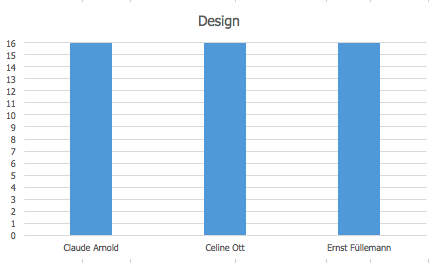
\includegraphics[width=0.8\textwidth]{./pictures/design.png}
16 Punkte Tot.

\subsection{Verständlichkeit}
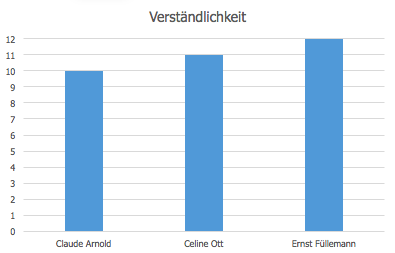
\includegraphics[width=0.8\textwidth]{./pictures/verstaendilchkeit.png}
12 Punkte Tot.

\subsection{Funktionalität}
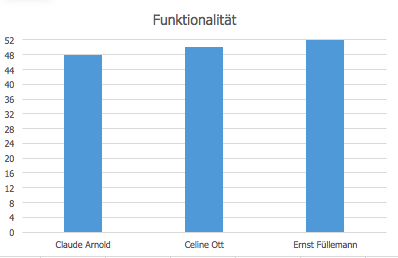
\includegraphics[width=0.8\textwidth]{./pictures/funktionalitaet.png}
52 Punkte Tot.

\subsection{Fehler}
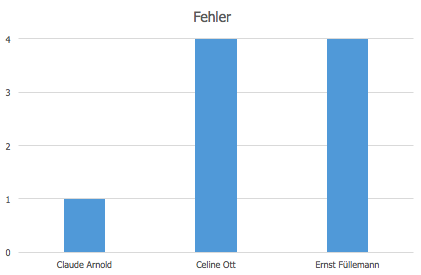
\includegraphics[width=0.8\textwidth]{./pictures/fehler.png}
4 Punkte Tot.

\subsection{Effizienz}
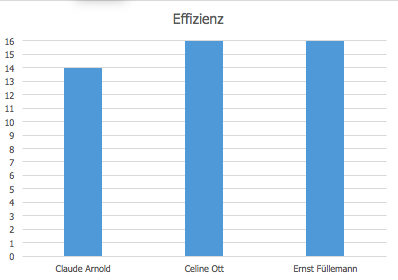
\includegraphics[width=0.8\textwidth]{./pictures/effizienz.png}
16 Punkte Tot.

\subsection{Zufriedenheit}
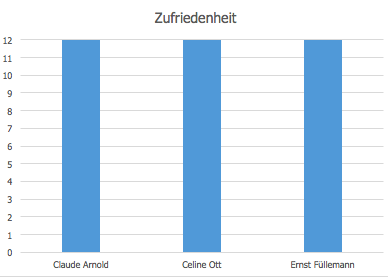
\includegraphics[width=0.8\textwidth]{./pictures/zufriedenheit.png}
12 Punkte Tot.

\subsection{Total}
Jeder Testperson kann Total 112 Punkte vergeben. \\
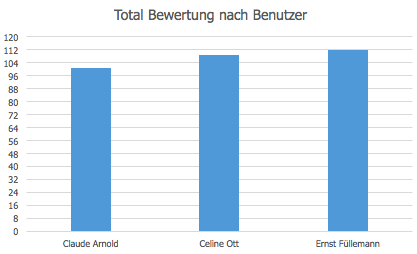
\includegraphics[width=0.8\textwidth]{./pictures/total_user.png}\\
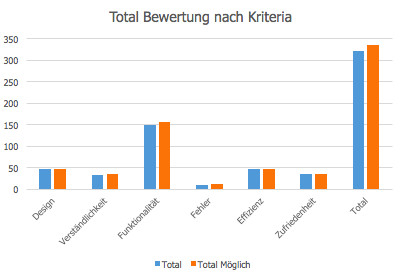
\includegraphics[width=0.8\textwidth]{./pictures/total_kriteria.png}
\begin{itemize}
\item Design: Total 3*16 = 48
\item Verständlichkeit: Total 3*12 = 36
\item Funktionalität: Total 3*52 = 156
\item Fehler: Total 3*4 = 12
\item Effizienz: Total 3*16 = 48
\item Zufriedenheit: Total 3*12 = 36
\end{itemize}

\subsubsection{Total Tabellarisch}
Siehe Legende weiter unten für Abkürzungserklärung.
\begin{table}[H]
\centering
    \begin{tabular}{@{} p{0.5cm} p{0.5cm} p{0.5cm} p{0.5cm} & p{0.5cm} & p{0.5cm} & p{0.5cm} & p{0.5cm} & p{0.5cm} & p{0.5cm} & p{0.5cm} & p{0.5cm} & p{0.5cm} & p{0.5cm} & p{0.5cm} @{}}\toprule    
    {Nr} & {D} & {DT} & {V} & {VT} & {F} & {FT} & {FE} & {FET} & {E} & {ET} & {Z} & {ZT} & {T} & {TT}\\ \midrule
    1 & 16 &16 &10 &12 &48 &52 &1 &4 &14 &16 & 12 &12 &101 &112   \\ \addlinespace
    2 & 16 &16 &11 &12 &50 &52 &4 &4 &16 &16 & 12 &12 &109 &112   \\ \addlinespace
    3 & 16 &16 &12 &12 &52 &52 &4 &4 &16 &16 & 12 &12 &112 &112   \\ 
    \bottomrule
    \end{tabular}
\caption{\textbf{Testprotokoll: Auswertung}}
\end{table}
\textbf{Legende}
\begin{itemize}
\item 1: Claude Arnold, 2: Celine Ott, 3: Ernst Füllemann
\item D: Design, DT: Design Total möglich
\item V: Verständlichkeit, VT: Verständlichkeit Total möglich
\item F: Funktionalität, FT: Funktionalität Total möglich
\item FE: Fehler, FET: Fehler Total möglich
\item E: Effizienz, ET: Effizienz Total möglich
\item Z: Zufiedenheit, ZT: Zufriedenheit Total möglich
\item T: Total, TT: Total möglich insgesamt 
\end{itemize}

\subsection{Fazit}
Wir sind mit den erzielten Resultaten sehr zufrieden. Das Programm scheint im Allgemeinen leicht bedienbar zu sein. Wie in den Requirements beschrieben werden elementare Netzwerkkenntnisse für das Benutzen der Software vorausgesetzt. Zusätzliche Features wie Aufzeichnung wären wünschenswert und würden die Software noch verbessern.


\end{document}

